\title{Lecture 2 - Numbers}
\frame{\titlepage}

%%%%%%%%%%%%%
\section{The Tale of Numbers}
\frame{\sectionpage}
%%%%%%%%%%%%%

\begin{frame}
\frametitle{Sets of Numbers}
Sets of numbers \pause 
\begin{block}{The set of natural numbers}
$\mathbb{N} = \{1,2,3,4,5,\ldots\} $  (aka. counting numbers)
\end{block}
\begin{block}{The set of integers}
$\mathbb{Z} = \{\ldots, -3,-2,-1,0,1,2,3,\ldots \}$ (includes negative numbers and zero)
\end{block}
\begin{block}{The set of rational numbers}
$\mathbb{Q} = \left\{ \frac{a}{b} \, | \, a,b \in \mathbb{Z} \text{ and } b \neq 0 \right\}$
\end{block}
\[ \mathbb{N} \subseteq \mathbb{Z} \pause \subseteq \mathbb{Q}\]
\end{frame}

\begin{frame}
\begin{figure}[h!]
\centering
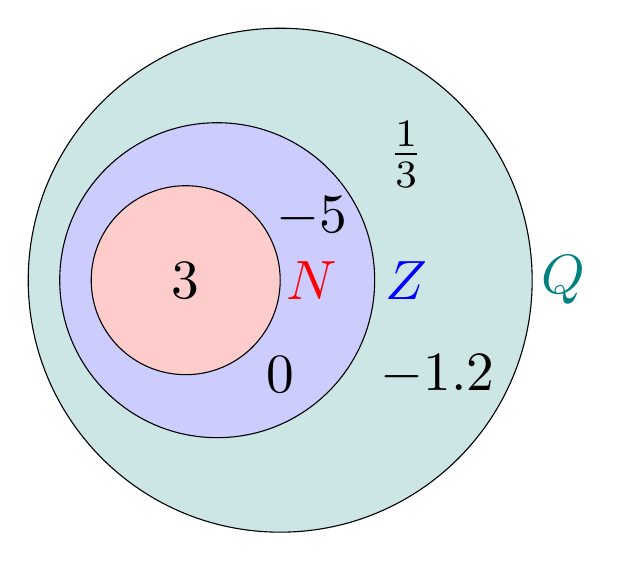
\begin{tikzpicture}[scale = 0.8, every node/.style = {scale = 2}]
\filldraw[fill = teal!20, draw = black] (0,0) circle (4cm);
\filldraw[fill = blue!20, draw = black] (-1,0) circle (2.5cm);
\filldraw[fill = red!20, draw = black] (-1.5,0) circle (1.5cm);
\node[teal] at (4.5,0) {$\mathbb{Q}$};
\node[blue] at (2,0) {$\mathbb{Z}$};
\node[red] at (0.5,0) {$\mathbb{N}$};
\node at (-1.5,0) {$3$};
\node at (0.5,1) {$-5$};
\node at (0,-1.5) {$0$};
\node at (2,2) {$\frac{1}{3}$};
\node at (2.5,-1.5) {$-1.2$};
\end{tikzpicture}
\caption{A diagram for natural numbers, integers, and rational numbers}
\end{figure}
\end{frame}

\begin{frame}
\frametitle{What is out there?}
\begin{block}{The set of irrational numbers}
 $\tilde{\mathbb{Q}}$  (not expressible as a fraction / non-repeating decimals) \pause
\end{block}
\begin{block}{The set of real numbers}
$\mathbb{R} = \mathbb{Q} \cup \tilde{\mathbb{Q}}$ 
(Numbers that can be represented as decimals) \pause
\end{block}
\[ \mathbb{N} \subset \mathbb{Z} \subset \mathbb{Q} \pause \subset \mathbb{R}\]
\end{frame}

\begin{frame}
\frametitle{What is in $\tilde{\mathbb{Q}}$?}
\pause Short answer: \pause pretty much everything. \pause

Long answer: 
\begin{block}{}
\begin{itemize}
\item Algebraic numbers (roots of polynomials) \pause 
\[ \sqrt{2}, \sqrt[3]{1.34}, \frac{1 - \sqrt{5}}{2}\] 
\item Computable numbers \pause
\[ e, \pi, \text{Euler's constant} , \ldots\] 
\item Non-computable numbers \pause
\[ \text{Chaitin's constant} \]
\end{itemize}
\end{block}
\end{frame}

\begin{frame}
\addfig{0.6}{non_computer_number_simba_meme}{Shadowy dark place, indeed}
\end{frame}

\begin{frame}
\frametitle{I NEED MORE!!!}
\begin{block}{The set of complex numbers}
\[\mathbb{C} = \{ a+bi\, |\, a,b \in \mathbb{R} \}\]
where $i = \sqrt{-1}$.
\end{block}
More? \pause

No! That's all the numbers! \pause
\end{frame}

\begin{frame}
\frametitle{ALL THE NUMBERS}
\addfig{0.8}{l03i05}{\href{https://www.youtube.com/watch?v=5TkIe60y2GI}{All the Numbers - Numberphile}}
\end{frame}

\begin{frame}
\frametitle{Famous Numbers} \pause
\begin{itemize}
\item Fibonacci number $F_n = F_{n-1} + F_{n-2}$  \pause
\begin{figure}[h!]
\centering

\includegraphics[width = 0.4\textwidth]{l03i01.png} \pause
\end{figure}
\item Triangular numbers $T_n = 1 + 2 + \cdots + n = \frac{n(n+1)}{2}$ \pause
\begin{figure}[h!]
\centering

\includegraphics[width = 0.2\textwidth]{l03i02.png} \pause

\includegraphics[width = 0.2\textwidth]{l03i03.png}
\end{figure}
\end{itemize}
\end{frame}

\begin{frame}
\frametitle{Exotic ``numbers''}
$\{ a+bi+cj+dk\, | \, a,b,c,d \in \mathbb{R} \}$ - Quaternion \pause
\begin{eqnarray*}
i^2 &=& j^2 = k^2 = -1 \\
ij &=& k \\
jk &=& i \\
ki &=& j
\end{eqnarray*} \pause
Useful in defining 3D rotations \pause
\begin{figure}[h!]
\centering

\includegraphics[width = 0.4\textwidth]{l03i04.png}
\end{figure}
\end{frame}

\begin{frame}
\begin{exercisebox}{}{}
Draw the Venn diagram for $\mathbb{N}, \mathbb{Z}, \mathbb{Q}, \mathbb{R}$ and put the following numbers in the appropriate section.
\[ -1, \sqrt{2}, 42, \pi, 0.8, \frac{1}{\pi}, 0.9999\ldots, \sqrt{0.25}\]
\end{exercisebox}
\end{frame}

%%%%%%%%%%%%%
\section{Common Keywords}
\frame{\sectionpage}
%%%%%%%%%%%%%

\begin{frame}
\frametitle{Recaps}
There are several commonly used keywords you should know (because, well, they are common.)
\begin{remark}{}
\begin{itemize}
\item Divisible, remainder
\item Prime vs. Composite \pause
\item Factor
\item Square, Cube, Fourth power, $\ldots$ \pause
\item Power or $n$  ($2^n, 3^n,$ etc.)
\end{itemize}
\end{remark}
\end{frame}

\begin{frame}
\frametitle{Divisibility}
\begin{defn}{}{}
Let $m$ and $k$ be integers. We say that \textbf{$m$ is divisible by $k$} if we can write $m$ as a product of $k$ and another integer. In other words, 
\[m = k \times n\]
for some integer $n$. We denote $k \mid m$.

Alternately, we say that $k$ divides $m$, or $k$ is a factor of $m$.
\end{defn}
\end{frame}

\begin{frame}
\frametitle{Remainder}
\begin{defn}{}{}
For any integers $m$ and $n$ (with $n > 0$), we can find unique integers $q$ and $r$ such that
\[m = q \times n + r\]
where $r$ is an integer from 0 to $n-1$. We call $q$ the \textbf{q}uotient and $r$ the \textbf{r}emainder.
\end{defn}

Note that when the remainder $r$ is zero, we have $m = q \times n$ and therefore $m$ is divisible by $n$.
\end{frame}

\begin{frame}{}
\begin{figure}[h!]
\centering
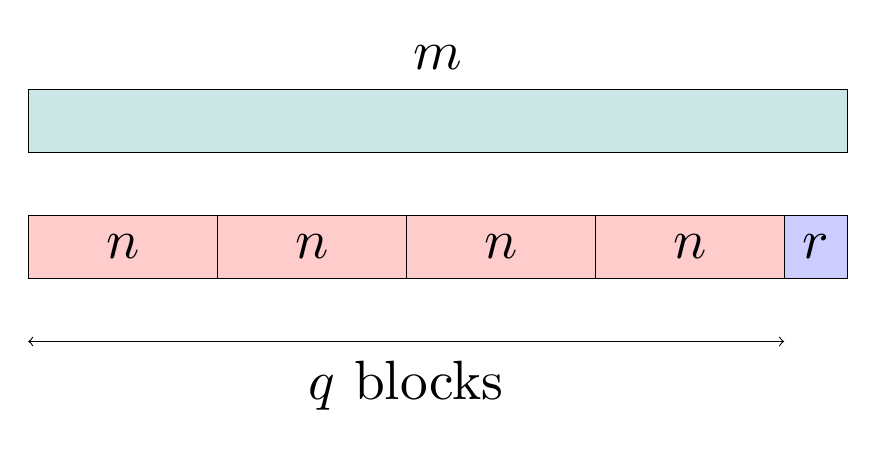
\begin{tikzpicture}[every node/.style={scale = 2}, scale = 0.8]
\filldraw[fill = teal!20, draw = black] (0,0) rectangle (13, 1);
\node at (6.5,1.5) {$m$};
\foreach \x in {0,3,6,9}
	\filldraw[fill = red!20, draw = black] (\x,-2) rectangle ({\x+3}, -1) node[pos = 0.5] {$n$};
\filldraw[fill = blue!20, draw = black] (12,-2) rectangle (13, -1) node[pos=0.5] {$r$};
\draw[<->] (0, -3) --+ (12,0) node[pos = 0.5, below] {$q$ blocks};
\end{tikzpicture}
\caption{A diagram for $m = q \times n + r$}
\end{figure}
\end{frame}

\begin{frame}[t]
\begin{ex}
For each pair of $m$ and $n$, find quotient $q$ and remainder $r$ such that $m = q \times n + r$ ($0 \le r < n$).
\begin{tasks}(2)
\task $m=10, n = 4$
\task $m=19, n = 3$
\task $m = 15, n = 3$
\task $m = 0, n = 5$
\end{tasks}
\end{ex}
\begin{sol}
\begin{tasks}(1)
\task $10 = 2 \times 4 + 2 \implies q = 2$ and $r = 2$.
\task $19 = 6 \times 3 + 1 \implies q = 6$ and $r = 1$.
\task $15 = 5 \times 3 + 0 \implies q = 5$ and $r = 0$.
\task $0 = 0 \times 5 + 0 \implies q = 0$ and $r = 0$.
\end{tasks}
\end{sol}
\end{frame}

\begin{frame}
\frametitle{Prime}
Notice two things: for any natural number $n$,
\begin{itemize}
\item $n$ is divisible by 1, because we can write $n = n \times 1$.
\item $n$ is divisible by itself, because we can write $n = 1 \times n$.
\end{itemize}
The numbers that \textbf{only} have these two divisors are interesting enough that we give them a name.
\begin{defn}{}{}
A natural number $n > 1$ which has only two distinct positive divisors (namely, 1 and itself) is called a \textbf{prime number}.

\medskip
If $n > 1$ is not a prime number, we call $n$ a \textbf{composite number}.
\end{defn}

\begin{remark}{}
1 is not a prime number! Because 1 has only one positive divisor.
\end{remark}
\end{frame}


\begin{frame}[t]
\begin{ex}
For each number, determine whether it is a prime number or a composite number.
\begin{tasks}(3)
\task $20$
\task $39$
\task $29$
\end{tasks}
\end{ex}
\begin{sol}
\begin{tasks}(1)
\task We can write $20 = 4 \times 5$. Thus, $20$ is divisible by another number besides 1 and itself, so it is a composite number.
\task We can write $39 = 13 \times 3$. Thus, $39$ is divisible by another number besides 1 and itself, so it is a composite number.
\task Testing divisibility by prime numbers up to $\sqrt{29} \approx 5.39$ (namely 2, 3, and 5), $29$ is not divisible by any of them. Thus, 29 is a prime number.
\end{tasks}
\end{sol}
\end{frame}


\begin{frame}
\frametitle{The Fundamental Theorem of Arithmetic}
\begin{thm}{}{}
Every integer $n > 1$ can be written as a product of prime powers in a unique way (up to the order of factors). In other words,
\[n = p_1^{k_1} p_2 ^{k_2} \cdots p_m^{k_m}\]
where $p_1, p_2, \ldots, p_m$ are distinct prime numbers, and $k_1, k_2, \ldots, k_m$ are positive integers.
\end{thm}

\end{frame}


\begin{frame}[t]
\begin{ex}
Express the following numbers as a product of prime numbers. 
\begin{tasks}(4)
\task 12
\task 40
\task 210
\task 256
\end{tasks}
\end{ex}
\begin{sol}
\begin{tasks}(1)
\task We can write 12 as $12 = 4 \times 3$, but $4$ is not a prime number. So, we need to use smaller factors and write 
\[12 = 2 \times 2 \times 3 = 2^2 \times 3.\]
\task $40 = 2 \times 2 \times 2 \times 5 = 2^3 \times 5$
\task $210 = 2 \times 3 \times 5 \times 7$
\task $256 = 2 \times 2 \times 2 \times 2 \times 2 \times 2 \times 2 \times 2 = 2^8$
\end{tasks}
\end{sol}
\end{frame}

\begin{frame}{Let's Play!}
\addfig{0.4}{prime_stone}{\href{https://boardgamegeek.com/boardgame/359327/prime-stone}{Prime Stone (designed by Kittiphan Wiboonsin}}{}
\end{frame}

\begin{frame}{How to play}
\begin{description}
\item[Goal] First to get 4 points win! (7 for full game)
\item[Set up] Two 2-coins, two 3-coins, two 5-coins, and a stone
\item Reveal 4 target cards
\item[Turn] Choose one of the three options
\begin{enumerate}
\item Draw 2 coins and place them in front of you
\item Choose 2 coins in front of you. Take the coin of value equal to their product. Return all three coins to your bag.
\item Choose 1 target card. Choose coins in front of you whose product equals to the value on the target card. Take the card and return those coins to your bag. Gain rewards (if any).
\end{enumerate}
\end{description}
\end{frame}

\begin{frame}
\frametitle{Square and Cube}
\begin{defn}{}{}
A natural number $n$ is a square if we can write $n$ as a square of another natural number. In other words, we can find a natural number $k$ such that $n = k^2$.
\medskip

A natural number $n$ is a cube if we can write $n$ as a cube of another natural number.
\end{defn}
These definitions are rarely used, but it's a handy keyword for the introductory course.
\end{frame}


\begin{frame}
\frametitle{Power of $k$}
\begin{defn}{}{}
A natural number $n$ is a power of $k$ if we can write $n$ as $k$ to the power of a natural number. In other words, we can find a natural number $m$ such that $n = k^m$.
\end{defn}
\begin{ex}
\begin{tasks}(1)
\task $16$ is a power of 2 because $16 = 2^4$.
\task $16$ is also a power of 4 because $16 = 4^2$.
\task $243$ is a power of 3 because $243 = 3^5$.
\task $-64$ is a power of $-4$ because $-64 = (-4)^3$.
\end{tasks}
\end{ex}
\end{frame}

\begin{frame}
\begin{exercisebox}{}{}
\begin{enumerate}
\item Given $m= 19, n =5$, find quotient $q$ and remainder $r$ such that $m = q \times n + r$ and $0 \leq r \leq n-1$.
\item Express 100 as a product of prime powers.
\item By trial and error, express 52 as a sum of a square and a cube.
\item By trial and error, express 25 as a sum of a power of 2 and a power of 3.
\end{enumerate}
\end{exercisebox}
\end{frame}

%%%%%%%%%%%%%
\section{Modulo}
\frame{\sectionpage}
%%%%%%%%%%%%%

\begin{frame}{Clock Arithmetic (Modulo 5)}
\begin{figure}[h!]
\centering
\begin{tikzpicture}[scale=1.1, >=Stealth]
% Draw main modulo circle
\draw[thick, teal!70!black] (0,0) circle (2cm);

% Nodes for 0, 1, 2, 3, 4
\foreach \i/\label in {0/0, 1/1, 2/2, 3/3, 4/4} {
  \pgfmathsetmacro{\angle}{90 - \i * 72}
  % Node circle
  \filldraw[fill=teal!15, draw=teal!80!black, thick] (\angle:2cm) circle (0.38cm);
  \node[font=\bfseries\Large, teal!90!black] at (\angle:2cm) {\label};
  
  % Curved arrow between consecutive numbers
  \draw[->, very thick, purple!80!black, shorten >=0.48cm, shorten <=0.48cm] 
    (\angle:2cm) arc[start angle=\angle, end angle=\angle-72, radius=2cm];
}

% Center label
\node at (0,0) [align=center] {\textbf{\Large Modulo 5}\\[3pt]\small Equivalence Classes:\\[1pt]\textcolor{teal!80!black}{\textbf{$\{0, 1, 2, 3, 4\}$}}};
\end{tikzpicture}
\caption{Modular arithmetic (mod 5) represented as positions on a circle}
\end{figure}
\end{frame}

\begin{frame}
\frametitle{Modulo}
\begin{defn}{}{}
Given integers $a,b$ and a positive integer $n$. If $n$ divides $a-b$, written as
\[ n \mid a-b, \]
then we write
\begin{equation} 
a \equiv b \pmod n
\end{equation}
This is read ``$a$ is congruent to $b$ modulo $n$''. We also say that $a$ and $b$ are in the same \textbf{equivalence class}.
\end{defn}
\end{frame}


\begin{frame}[t]
\begin{ex}
Given an integer $a$ and a modulo $n$, find 3 other integers that are congruent to $a \pmod n$.
\begin{tasks}(3)
\task $2 \pmod 5$
\task $20 \pmod 9$
\task $-11 \pmod 3$
\end{tasks}
\end{ex}
\begin{sol}
\begin{tasks}(1)
\task $7,12,17$ are all congruent to $2 \pmod 5$ because $7-2, 12-2, 17-2$ are all divisible by 5.
\task $2, 11, 29$ are all congruent to $20 \pmod 9$ because $2-20, 11-20, 29-20$ are all divisible by 9.
\task $-8, -5, -2$ are all congruent to $-11 \pmod 3$ because $(-11)-(-8), (-11)-(-5), (-11)-(-2)$ are all divisible by 3.
\end{tasks}
\end{sol}
\end{frame}

\begin{frame}
\frametitle{Properties of Modulo}
\begin{prop}{}{}
Let $a,b,c,d,k$ be integers and $n$ be a positive integer. Suppose that $a \equiv b \pmod n$ and $c \equiv d \pmod n$. Then, the following operations preserve congruence modulo $n$:
\begin{itemize}
\item Addition by a constant: $a + k \equiv b + k \pmod n$.
\item Multiplication by a constant: $a \times k \equiv b \times k \pmod n$.
\item Addition: $a + c \equiv b+d \pmod n$.
\item Multiplication: $a \times c \equiv b \times d \pmod n$.
\end{itemize}
\end{prop}
\end{frame}


\begin{frame}[t]
\begin{ex}
Compute the following
\begin{tasks}(2)
\task $22 + 12 \mod 7$ 
\task $22 \times 12 \mod 7$ 
\end{tasks}
\end{ex}
\begin{sol}
\begin{tasks}(1)
\task We can either 
\begin{itemize}
\item Find the sum directly, which is $22+12 \equiv 34 \equiv 6 \mod 7$.
\item Reduce each term in mod 7 so that the sum is smaller. Since $22 \equiv 1 \mod 7$ and $12 \equiv 5 \mod 7$, we have $22 + 12 \equiv 1 + 5 \equiv 6 \mod 7$
\end{itemize}

\task We can either
\begin{itemize}
\item Find the product directly, which is $22 \times 12 \equiv 264 \equiv 5 \mod 7$.
\item Reduce each term in mod 7 so that product is smaller.  Since $22 \equiv 1 \mod 7$ and $12 \equiv 5 \mod 7$, we have $22 \times 12 \equiv 1 \times 5 \equiv 5 \mod 7$
\end{itemize}
\end{tasks}
\end{sol}
\end{frame}


\begin{frame}[t]
\begin{ex}
Compute the following
\begin{tasks}(2)
\task $1233 \times 3434 \mod 10$
\task $3^{100} \mod 8$
\end{tasks}
\end{ex}
\begin{sol}
\begin{tasks}(1)
\task Finding the product directly might take more time, so here we use the property. Since $1233 \equiv 3 \mod 10$ and $3434 \equiv 4 \mod 10$, then we have $1233 \times 3434 \equiv 3 \times 4 \equiv 12 \equiv 2 \mod 10$.

\task This is an example where it is not advisable to compute the number first. We notice that $3^2 \equiv 9 \equiv 1 \mod 8$, so
\[ 3^{100} \equiv 3^2 \times 3^2 \times \cdots \times 3^2 \equiv 1 \times 1 \times \cdots \times 1 \equiv 1 \mod 8\]
Hence, $3^{100} \equiv 1 \mod 8$.
\end{tasks}
\end{sol}
\end{frame}

\begin{frame}
\begin{exercisebox}{}{}
\begin{enumerate}
\item Find three pairs of numbers from $-5,0,2,7,14,24$ such that for each pair $a,b$, we have $a \equiv b \mod 12$.
\item Use properties of modulo to compute the following 
\begin{tasks}(2)
\task $100 + 200 \mod 9$
\task $100 \times 200 \mod 11$
\task $2022 \times 2564 \mod 10$
\task $4^{100} \mod 15$
\end{tasks}
\end{enumerate}
\end{exercisebox}
\end{frame}



%%%%%%%%%%%%%
\section{Number Bases}
\frame{\sectionpage}
%%%%%%%%%%%%%

\begin{frame}
\frametitle{Motivation}
What do you mean when you write the number 
\[99?\]

\addfig{0.8}{number_base_intro}{\href{https://www.youtube.com/watch?v=2SUvWfNJSsM&ab_channel=3Blue1Brown}{Binary, Hanoi and Sierpinski, part 1}}{}
\end{frame}


\begin{frame}
\frametitle{}
\begin{defn}{}{}
A base $m$ number is written in the form 
\[(a_k a_{k-1} a_{k-2} \cdots a_0)_m\]
where $k$ is the number of digits and each $a_k, a_{k-1}, \cdots, a_0$ is an integer from 0 to $m-1$ and $a_k$ is non-zero.
\end{defn}
\begin{ex}
$(11)_4$ is a base 4 number and $(2021)_5$ is a base 5 number.
\medskip

$(023)_4$ is not a valid number because the leading digit is zero. $(150)_5$ is not a valid number because a base 5 number needs all digits to be less than 5.
\end{ex}
\end{frame}

\begin{frame}
\frametitle{Converting base-$m$ numbers to base 10}
\begin{defn}{}{}
Let $n = (a_k a_{k-1} a_{k-2} \cdots a_0)_m$ where $n$ is the number written in base 10. Then, we have the formula
\begin{equation}
n = a_k \times (m^k) + a_{k-1} \times (m^{k-1}) + \cdots + a_1 \times m + a_0.
\end{equation}
\end{defn}
\end{frame}


\begin{frame}[t]
\begin{ex}
Write the following numbers in base 10
\begin{tasks}(3)
\task $(1010)_2$
\task $(210)_3$
\task $(103)_5$
\end{tasks}
\end{ex}
\begin{sol}
\begin{tasks}(1)
\task $(1010)_2 = 1 \times 2^3 + 0 \times 2^2 + 1 \times 2^1 + 0 = 8 + 0 + 2 + 0 = 10$
\task $(210)_3 = 2 \times 3^2 + 1 \times 3^1 + 0 = 18 + 3 = 21$
\task $(103)_5 = 1 \times 5^2 + 0 \times 5^1 + 3 = 25 + 0 + 3 = 28$
\end{tasks}
\end{sol}
\end{frame}


\begin{frame}
\frametitle{Digits in base higher than 10}
We know that each digit is between $0$ and the base itself. What do we do if we work in base 16?

\begin{defn}{}{}
If the base is higher than 10, we use English letters. \pause
\[ A = 10, B = 11, C = 12, D = 13, E = 14, F = 15 \]
\end{defn}

Popular bases are base 12 with digits $0,1,2,\ldots, 9,A,B$ and base 16 with digits $0,1,2,\ldots,9,A,B,C,D,E,F$.
\end{frame}


\begin{frame}[t]
\begin{ex}
Write the following numbers in base 10
\begin{tasks}(3)
\task $(1A)_{12}$
\task $(B3)_{16}$
\task $(A0E)_{16}$
\end{tasks}
\end{ex}
\begin{sol}
\begin{tasks}(1)
\task $(1A)_{12} = 1 \times (12) + 10 = 22$
\task $(B3)_{16} = 11 \times (16) + 3 = 179$
\task $(A0E)_{16} = 10 \times (16^2) + 0 \times (16) + 14 = 2560 + 0 + 14 = 2574$
\end{tasks}
\end{sol}
\end{frame}

\begin{frame}
\frametitle{Converting base-10 numbers to any base}
\begin{defn}{Division Algorithm}{}
Let $n$ and $m$ be positive integers ($m > 1$). We can write $n$ in base $m$ using the following division algorithm:
\begin{enumerate}
\item Divide $n$ by $m$ and write $n = m \times q_1 + r_1$, where $q_1$ is the quotient and $r_1$ is the remainder ($0 \leq r_1 \leq m-1$).
\item Repeat for $q_1$: Write $q_1 = m \times q_2 + r_2$ where $q_2$ is the quotient and $r_2$ is the remainder ($0 \le r_2 \le m-1$).
\item Stop when $q_k = 0$ (i.e. we cannot divide further).
\item The base $m$ representation is $n = (r_k r_{k-1} \ldots r_2 r_1)_m$.
\end{enumerate}
\end{defn}
\end{frame}


\begin{frame}[t]
\begin{ex}
Write 13 in base 2
\end{ex}
\begin{sol}
\begin{itemize}
\item Divide 13 by 2 and write $13 = 2 \times 6 + 1$. We have $q_1 = 6$ and $r_1 = 1$.
\item Divide 6 by 2 and write $6 = 2 \times 3 + 0$. We have $q_2 = 3$ and $r_2 = 0$.
\item Divide 3 by 2 and write $3 = 2 \times 1 + 1$. We have $q_3 = 1$ and $r_3 = 1$.
\item Divide 1 by 2 and write $1 = 2 \times 0 + 1$. We have $q_4 = 0$ and $r_4 = 1$.
\end{itemize}
Now that $q_4 = 0$, we stop and conclude that $13 = (1101)_2$.
\end{sol}
\end{frame}

\begin{frame}{}
\begin{figure}[h!]
\centering
\begin{tikzpicture}
\node at (0,1) {$m$};
\node at (1, 1) {$q$};
\node at (2.5,1) {$r$};
\foreach \y / \q / \r in {0/13/1, -1/6/0, -2/3/1, -3/1/1}
{
	\node at (0, \y) {$2$};
	\node at (1, \y) {$\q$};
	\node at (2.5,{\y-1}) {$\r$};
	\draw (0.5,{\y+0.4}) --++ (0, -0.8) --+ (1.5,0);
}
\node at (1,-4) {0};
\draw[double] (0.5, -4.4) --+ (1.5,0);
\draw[->] (3, -4) -- (3,-1) node[right] {$(1101)_2$};
\end{tikzpicture}
\caption{Division algorithm for finding $13$ in base $2$}
\end{figure}
\end{frame}

\begin{frame}[t]
\begin{ex}
Write 78 in base 4
\end{ex}
\begin{sol}
\begin{itemize}
\item Divide 78 by 4 and write $78 = 4 \times 19 + 2$. We have $q_1 = 19$ and $r_1 = 2$.
\item Divide 19 by 4 and write $19 = 4 \times 4 + 3$. We have $q_2 = 4$ and $r_2 = 3$.
\item Divide 4 by 4 and write $4 = 4 \times 1 + 0$. We have $q_3 = 1$ and $r_3 = 0$.
\item Divide 1 by 4 and write $1 = 4 \times 0 + 1$. We have $q_4 = 0$ and $r_4 = 1$.
\end{itemize}
Now that $q_4 = 0$, we stop and conclude that $78 = (1032)_4$.
\end{sol}
\end{frame}

\begin{frame}{}
\begin{figure}[h!]
\centering
\begin{tikzpicture}
\node at (0,1) {$m$};
\node at (1, 1) {$q$};
\node at (2.5,1) {$r$};
\foreach \y / \q / \r in {0/78/2, -1/19/3, -2/4/0, -3/1/1}
{
	\node at (0, \y) {$4$};
	\node at (1, \y) {$\q$};
	\node at (2.5,{\y-1}) {$\r$};
	\draw (0.5,{\y+0.4}) --++ (0, -0.8) --+ (1.5,0);
}
\node at (1,-4) {0};
\draw[double] (0.5, -4.4) --+ (1.5,0);
\draw[->] (3, -4) -- (3,-1) node[right] {$(1032)_4$};
\end{tikzpicture}
\caption{Division algorithm for finding $78$ in base $4$}
\end{figure}
\end{frame}

\begin{frame}[t]
\begin{ex}
Write 175 in base 16
\end{ex}
\begin{sol}
\begin{itemize}
\item Divide 175 by 16 and write $175 = 16 \times 10 + 15$. We have $q_1 = 10$ and $r_1 = 15$. In base 16, $r_1$ corresponds to F.
\item Divide 10 by 16 and write $10 = 16 \times 0 + 10$. We have $q_2 = 0$ and $r_2 = 10$. In base 16, $r_2$ corresponds to A.
\end{itemize}
Now that $q_2 = 0$, we stop and conclude that $175 = (\text{AF})_{16}$.
\end{sol}
\end{frame}


\begin{frame}{}
\begin{figure}[h!]
\centering
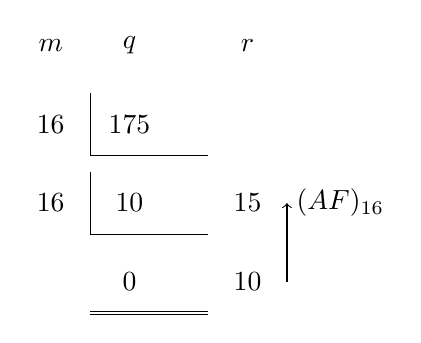
\begin{tikzpicture}
\node at (0,1) {$m$};
\node at (1, 1) {$q$};
\node at (2.5,1) {$r$};
\foreach \y / \q / \r in {0/175/15, -1/10/10}
{
	\node at (0, \y) {$16$};
	\node at (1, \y) {$\q$};
	\node at (2.5,{\y-1}) {$\r$};
	\draw (0.5,{\y+0.4}) --++ (0, -0.8) --+ (1.5,0);
}
\node at (1,-2) {0};
\draw[double] (0.5, -2.4) --+ (1.5,0);
\draw[->] (3, -2) -- (3,-1) node[right] {$(AF)_{16}$};
\end{tikzpicture}
\caption{Division algorithm for finding $175$ in base $16$}
\end{figure}
\end{frame}

\begin{frame}
\begin{exercisebox}{}{}
\begin{enumerate}
\item Compute the following numbers (i.e. convert them to base 10).
\begin{tasks}(3)
\task $(10101)_2$
\task $(3412)_6$
\task $(EA)_{16}$
\end{tasks}
\item Write the following numbers in the given base.
\begin{tasks}(3)
\task 20 in base 3
\task 100 in base 2
\task 50 in base 16
\end{tasks}
\end{enumerate}
\end{exercisebox}
\end{frame}

